\pdfpagewidth=8.5in
\pdfpageheight=11in

\documentclass{sig-alternate}
\usepackage[utf8]{inputenc}
\usepackage[T1]{fontenc}
\usepackage{microtype}

\usepackage{url}
\usepackage{amsmath}
\usepackage{graphicx}
\usepackage{subfigure}
\usepackage{threeparttable}
\usepackage{pdflscape}
\usepackage{array}
\usepackage{color}

\usepackage{flushend}

\clubpenalty = 10000
\widowpenalty = 10000
\displaywidowpenalty = 10000

\begin{document}

\conferenceinfo{MSR}{'15, May 16 – 17, 2015, Florence, Italy}
\CopyrightYear{2015}
\crdata{978-1-4503-2863-0/14/05}

\title{Generating the Blueprints of the Java Ecosystem}

\numberofauthors{5}

\def\aueb{\textsuperscript{*}}
\def\columbia{\textsuperscript{\ddag}}
\def\run{\textsuperscript{\dag}}

\author{
  Vassilios Karakoidas\aueb \and Dimitris Mitropoulos\columbia \and Georgios Gousios\run \and Diomidis Spinellis\aueb \and Panos Louridas\aueb\\
  \begin{tabular}{c}
   \affaddr{\aueb Dept of Management Science and Technology}\\
   \affaddr{Athens University of Economics and Business}\\
   \affaddr{Athens, Greece}\\
   \email{\{bkarak,dds,louridas\}@aueb.gr}\\
  \end{tabular}
  \centering
  \begin{tabular}{cc}
   \affaddr{} & \affaddr{\columbia Computer Science Department}\\
   \affaddr{Radboud University Nijmegen} & \affaddr{Columbia University}\\
   \affaddr{Nijmegen, the Netherlands} & \affaddr{New York, United States}\\
   \email{g.gousios@cs.ru.nl} & \email{dimitro@cs.columbia.edu}\\
  \end{tabular}
}

\maketitle
\begin{abstract}
Examining a large number of software artifacts can provide
the research community with data regarding quality and design.
We present a dataset obtained by statically analyzing
22730 {\sc jar} files taken from the Maven
central archive, which is the de-facto application library repository for the Java ecosystem. For our analysis
we used three popular static analysis tools
that calculate metrics regarding object-oriented design,
program size, and package design.
The dataset contains the metrics results that every tool
reports for every selected {\sc jar} of the
ecosystem. Our dataset can be used to produce interesting
research results, such as measure the domain-specific language usage.
\end{abstract}

\category{D.2.8}{Software Engineering}{Metrics}[Product metrics]

\terms{Static Analysis, Software Metrics}

\keywords{Java, Software Metrics, Chidamber and Kemerer, Maven}

\section{Introduction}
\label{sec:intro}

We present a dataset that contains popular metrics, calculated from the analysis of a large collection of software artifacts written in Java. All artifacts were taken from the {\it Maven Central Repository}~\cite{MAVEN}.

Maven is a build automation tool used primarily for Java projects, and it is maintained by the Apache Software Foundation~\cite{MAVEN}. To describe the software project being built, its dependencies, and the build order, Maven uses {\sc xml}. The central repository contains more than 400,000 {\sc jar}s, in a variety of programming languages such as Java, Clojure, Groovy, and Scala. All supported languages use the {\sc jvm} platform as their runtime environment. To build a software component, it dynamically downloads Java libraries and other plug-ins from the Maven central repository, and stores them in a local cache. The repository can be updated with new projects and also with new versions of existing projects that can depend on other versions.

To analyze the projects coming from Maven repository, we used the following tools: a) {\sc ckjm} \cite{Spi05g}, b) {\sc jd}epend~\cite{JDEPEND}, and c) {\sc clmt}~\cite{SGKL09}. All tools focus on three main aspects of a software system, namely: object-oriented design, program size, and package design. Such aspects are considered very important because they provide quantifiable information about the quality and structure of a software component.

In this paper we present: a) the construction process to obtain the collection of the metrics results that the three aforementioned tools produced for 22730 {\sc jar}s, b) our dataset and c) how researchers and practitioners can use the dataset and produce meaningful results.

\section{Dataset Construction Process}
\label{sec:data}

\begin{figure}
\centering
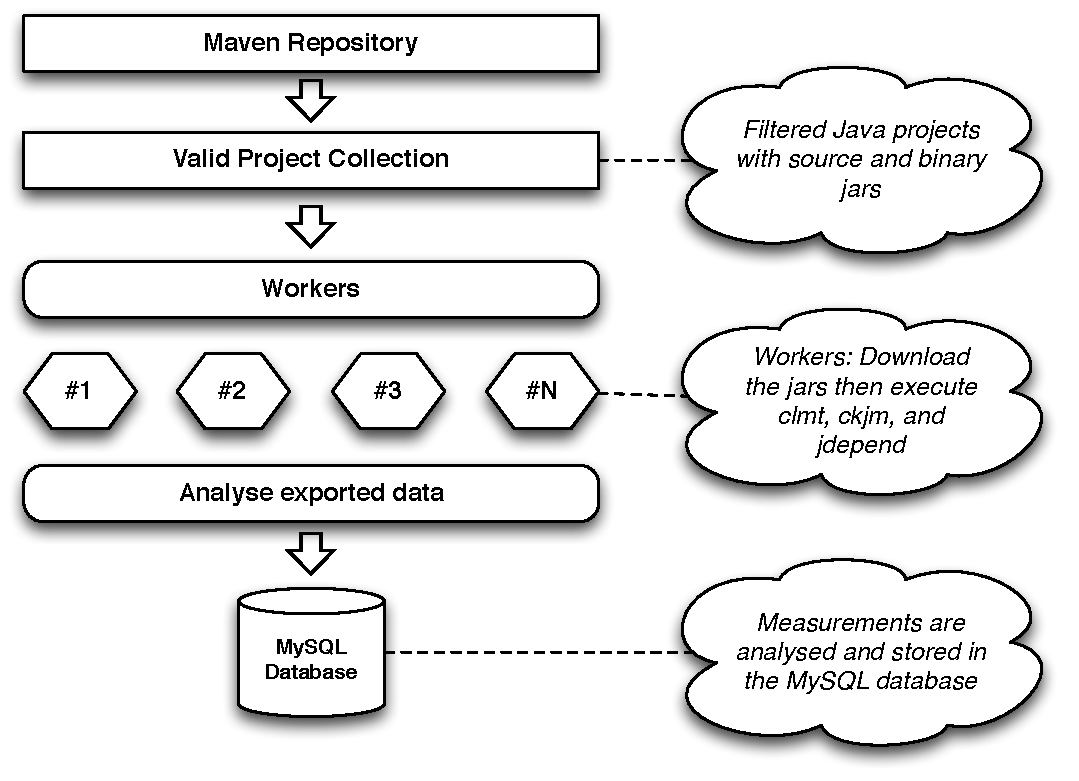
\includegraphics[scale=0.45]{import-process}
\caption{The dataset construction process}
\label{fig:dataset-construction}
\end{figure}

The dataset construction process is illustrated in Figure~\ref{fig:dataset-construction}. In general, it follows the same methodology presented in reference \cite{MKLGS14}.

Initially, a snapshot of the Maven repository was downloaded locally. The repository contains various projects that contain several versions. In our experiment, we only used Java projects. For every Java project all versions were filtered out and only the latest was kept. The process to identify them was the following; Every project consists of two {\sc jar} files, one that contains a compiled version of the project and one that contains the source code. The projects that did not had both binary and source {\sc jar}s, were excluded from the experiment. When the source {\sc jar} file was downloaded, it was scanned for Java source files. If the source files were present in the archive, then the project was flagged as a valid Java project.

When the selection process was finished, we created a series of processing tasks based on the selected {\sc jar}s, and added them to a task queue mechanism. Then we executed a number of workers that checked out tasks from the queue, applied the static analysis tools on each {\sc jar} and stored the results to the data repository (a {\sc m}y{\sc sql} database system). The workers were written in Python. In addition, there were several shell scripts (bash) that performed several checks and sanitisation tasks (e.g. checking for malformed results). The tools that were applied on every {\sc jar} were the following:

\begin{itemize}
  \item \textbf{CKJM-ext} \textit{(ckjm)}~\cite{Spi05g}; which calculates many software metrics, including the \textit{Chidamber and Kemmerer} set of object-oriented metrics \cite{CHKE94}. The version of the tool that we used for this experiment can be found in GitHub~\cite{CKJM}.

  \item \textbf{JDepend} \textit{(jdep)}~\cite{JDEPEND}; a tool that analyses {\sc jar} files that contain compiled Java classes and calculates a series of design metrics.

  \item \textbf{CLMT} \textit{(clmt)}~\cite{SGKL09}; which stands for \textit{cross-language metric tool} and analyses the source code of several languages in order to calculate a series of size metrics.
\end{itemize}

\begin{table}
\centering
\caption{The selected Maven projects' size metrics}
\label{tbl:oss-size-metrics}
\begin{tabular}{l r}
 \hline
\textbf{Metric} & \textbf{Value}\\
\hline
Project Count & 11,365\\
File Count & 449,213\\
Package Count & 59,436\\
Lines of Code & 74,565,772\\
Source Lines of Code & 40,921,287\\
Comment Lines of Code & 25,268,959\\
Number of Classes & 370,518\\
Number of Interfaces & 66,352\\
Number of Enumerations & 9,879\\
Measurement Count & 32,844,836\\
\hline
\end{tabular}
\end{table}

Table \ref{tbl:oss-size-metrics} presents several size metrics for our dataset. It includes 11,365 projects, with more than 74 million lines of code and almost 33 million unique measurements. Table~\ref{tbl:class-selected-metrics}, \ref{tbl:method-selected-metrics}, \ref{tbl:package-selected-metrics}, and \ref{tbl:size-selected-metrics} present the key metrics that are calculated and stored in the dataset. Each tool focuses on a different aspect of a software system; \textit{ckjm} focuses on object-oriented design metrics \cite{LOKI94}, \cite{CHKE94}, \textit{jdepend} on package design, while \textit{clmt} focuses on program size metrics. Several metrics are calculated by more than one tool, like \textit{cyclomatic complexity} \cite{cabe76}, which is calculated by both \textit{clmt} and \textit{ckjm}. Both calculations are available in the database.

A series of newly introduced metrics were also stored in the database. Such metrics can count the usage of specific {\sc dsl} application libraries in a software project and they are included in the Table~\ref{tbl:size-selected-metrics}. The methodology to identify and calculate the {\sc dsl} metrics was the following: A set of standard {\sc dsl} application libraries was identified, and the source was scanned for specific \textit{import} statements (e.g. \textit{java.util.regex}). These statements indicated that the standard package that implements regular expressions was used, thus regular expressions were used in the project. Build files or other resources that may contain {\sc dsl}s were not included. One final assumption was also made; if {\sc xp}ath or {\sc xslt} were found in the source code, then the project would be marked as a project that utilizes {\sc xml}. This is because both languages are used for query and transformations on {\sc xml} {\sc dom} trees. Table \ref{tbl:dsl-list} lists the selected {\sc dsl}s application libraries. Note that we focused on libraries that were included as part of the Java {\sc sdk}.

\begin{table}
\centering
\caption{List of selected DSL application libraries}
\label{tbl:dsl-list}
\begin{tabular}{l l}
 \hline
\textbf{DSL} & \textbf{Java Package}\\
\hline
Regular Expressions & \verb|java.util.regex|\\
XML & \verb|javax.xml|, \verb|org.w3c| and \verb|org.xml|\\
SQL & \verb|java.sql| and \verb|javax.sql|\\
XPath & \verb|java.xml.xpath|\\
XSLT & \verb|javax.xml.transform|\\
RTF & \verb|javax.swing.text.rtf|\\
HTML & \verb|javax.swing.text.html|\\
\hline
\end{tabular}
\end{table}

In Section~\ref{sec:dsl}, we describe an experiment based on these metrics. The experiment measures the popularity of {\sc dsl} usage for the dataset and therefore for the Java ecosystem in general.

\begin{table}
\centering
\caption{Class Design Metrics}
\label{tbl:class-selected-metrics}
\begin{tabular}{l l}
 \hline
\multicolumn{2}{l}{\textit{\textbf{Class Design}}}\\
\hline
Depth Of Inheritance Tree & \textit{ckjm}\\
Coupling Between Objects & \textit{ckjm}\\
Weighted Methods Per Class & \textit{ckjm}\\
Response For Class & \textit{ckjm}\\
Lack Of Cohesion In Methods & \textit{ckjm}\\
Number Of Children & \textit{ckjm}\\
Attribute Hiding Factor & \textit{clmt}\\
Coupling Between Methods & \textit{ckjm}\\
Average Method Complexity & \textit{ckjm}\\
Cohesion Among Methods of Class & \textit{ckjm}\\
Data Access Metric & \textit{ckjm, clmt}\\
Inheritance Coupling & \textit{ckjm}\\
Lack Of Cohesion In Methods3 & \textit{ckjm}\\
Measure Of Aggregation & \textit{ckjm}\\
Measure Of Functional Abstraction & \textit{ckjm}\\
Number of Attributes & \textit{clmt}\\
Method Hiding Factor & \textit{clmt}\\
\hline
\end{tabular}
\end{table}

\begin{table}
\centering
\caption{Method Design Metrics}
\label{tbl:method-selected-metrics}
\begin{tabular}{l l}
 \hline
\multicolumn{2}{l}{\textit{\textbf{Method Design}}}\\
\hline
Number of Method Parameters & \textit{clmt}\\
Number of Methods & \textit{clmt, ckjm}\\
McCabe Cyclomatic Complexity & \textit{ckjm, clmt}\\
\hline
\end{tabular}
\end{table}

\begin{table}
\centering
\caption{Method Design Metrics}
\label{tbl:package-selected-metrics}
\begin{tabular}{l l}
 \hline
\multicolumn{2}{l}{\textit{\textbf{Package Design}}}\\
\hline
Number of Concrete Classes & \textit{jdep}\\
Afferent Couplings & \textit{jdep, ckjm}\\
Efferent Couplings & \textit{jdep, ckjm}\\
Instability & \textit{jdep}\\
Abstractness & \textit{jdep}\\
Distance Main Sequence & \textit{jdep}\\
\hline
\end{tabular}
\end{table}

\begin{table}
\centering
\caption{Program Size Metrics}
\label{tbl:size-selected-metrics}
\begin{tabular}{l l}
 \hline
\multicolumn{2}{l}{\textit{\textbf{Program Size Metrics}}}\\
\hline
Number of Classes & \textit{clmt, ckjm, jdep}\\
Number of Enumerations & \textit{clmt, ckjm}\\
Number of Interfaces & \textit{clmt, ckjm}\\
Module Count & \textit{clmt, ckjm}\\
Comments Lines Of Code & \textit{clmt}\\
Lines Of Code & \textit{clmt, ckjm}\\
Source Lines Of Code & \textit{clmt}\\
Function Oriented Code & \textit{clmt}\\
DSL Usage Count & \textit{clmt}\\
RTF Usage Count & \textit{clmt}\\
Regex Usage Count & \textit{clmt}\\
HTML Usage Count & \textit{clmt}\\
XPath Usage Count & \textit{clmt}\\
XSLT Usage Count & \textit{clmt}\\
XML Usage Count & \textit{clmt}\\
SQL Usage Count & \textit{clmt}\\
File Count & \textit{clmt}\\
\hline
\end{tabular}
\end{table}

\section{Database Structure}
\label{sec:db}

Figure~\ref{fig:database-schema} illustrates the database schema. It consists of five tables; \textit{measurement}, \textit{category}, \textit{identifiers}, \textit{measurement\_type}, and \textit{project}. The central database table is \textit{measurement}, which holds the measurement values. The other tables are used for normalization.

Metrics are divided into six categories that define their scope; \textit{module}, \textit{class}, \textit{method}, \textit{code unit}, and \textit{project-wide}. These values are stored in \textit{category} database table.

The descriptive names for each metric are stored in the \textit{measurement\_type} database table. There are 65 metrics available in the dataset. The names are composed by the actual metric name and the tool that was used to calculate them e.g. \textit{McCabe\_clmt} denotes that the metric name is the McCabe cyclomatic complexity from the \textit{clmt} tool, while \textit{McCabe\_ckjm} means that it is the same metric calculated by the \textit{ckjm} tool.

Filenames, methods, classes and package names along with other identifiers are stored in the \textit{identifiers} table. Note that each measurement has a related filename and a related identifier that points to a software element e.g. the \textit{afferent coupling} metric for the module in the directory ``com/scalagent/jmx'' is related with the identifier \textit{com.scalagent.jmx}.

Finally, the database table \textit{project} contains the related project identifiers, directly extracted from the maven repository.

\begin{figure*}
\centering
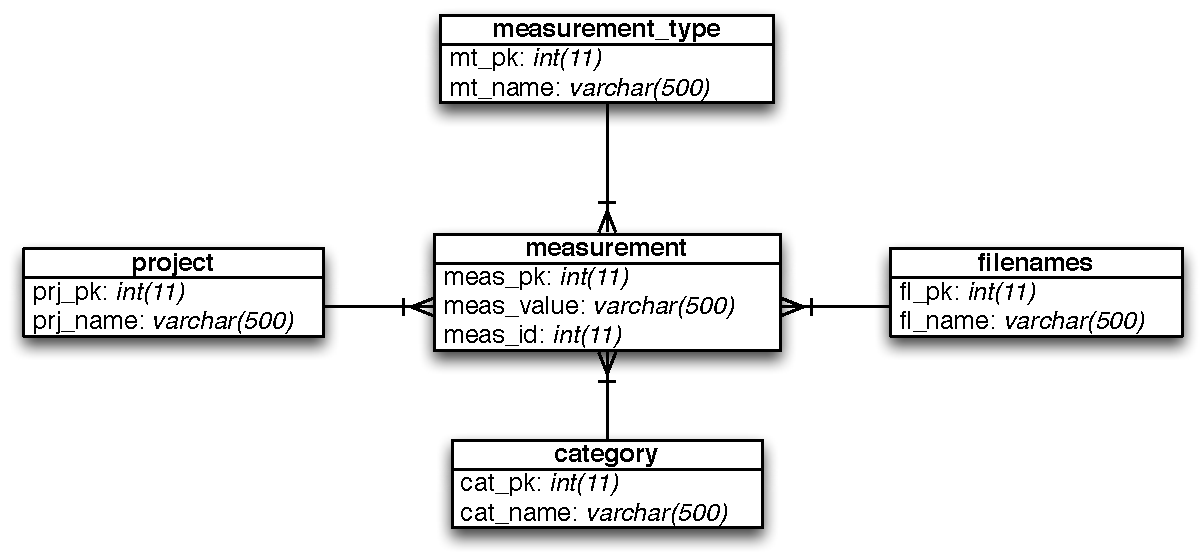
\includegraphics[scale=0.7]{database-schema}
\caption{The database schema}
\label{fig:database-schema}
\end{figure*}

\section{Research Opportunities}
\label{sec:research-opportunities}

The measurements provided by this dataset, can be used both by researchers and practitioners to validate their ideas. Researchers can use the data to experiment with new quality models, or just validate them in real projects. Practitioners who develop tools that calculate metrics can use the dataset to validate if their tools work correctly.

The dataset includes the {\sc dsl}-related metrics, which quantifies the usage of basic {\sc dsl} application libraries that are already shipped with the Java {\sc sdk}. These kind of metrics, can be really useful for researchers that focus on {\sc dsl} embedding, or study {\sc dsl} usage patterns \cite{KARA14}.

In addition, this dataset can be used side-by-side with the ones presented by Mitropoulos et al.~\cite{HP04} and Raemaekers et al.~\cite{RDV13} in order to examine the datasets for metric correlations, since these dataset also analysed projects from the Maven repository.

\section{Experimenting with the Dataset}
\label{sec:dsl}

\begin{table}
\centering
\caption{DSL Usage Combinations Ranking}
\label{tbl:dsl-top-usage}
\begin{tabular}{l r}
 \hline
\textbf{DSLs} & \textbf{Count}\\
\hline
XML & 1,561\\
Regex & 909\\
SQL & 493\\
XML, XSLT & 475\\
Regex, XML, XSLT & 158\\
Regex, XML & 303\\
SQL, XML & 162\\
Regex, SQL & 116\\
Regex, SQL, XML, XSLT & 80\\
Regex, SQL, XML & 71\\
SQL, XML, XSLT & 54\\
XML, XPath & 50\\
\hline
\end{tabular}
\end{table}

The initial goal of this experiment was to provide quantifiable results that are indicative regarding the usage of each {\sc dsl} for the Java ecosystem. The related metrics can be found in the database table named \textit{measuremnt\_type}, these are: \textit{RTFUsage\_clmt}, \textit{RegexUsage\_clmt},
\textit{HTMLUsage\_clmt}, \textit{HTMLUsage\_clmt}, \textit{XPathUsage\_clmt}, \textit{XSLTUsage\_clmt}, \textit{XMLUsage\_clmt}, \textit{SQLUsage\_clmt}, and \textit{DSLCount\_clmt}. With a python script that analyses the measurements stored in the database, we produced Table~\ref{tbl:dsl-top-usage}, which lists popular {\sc dsl} usage combinations for the dataset. We see that {\sc xml} is the big winner with 1561 occurrences in 11365 projects (13\%). Regular expressions are second most popular with 909 occurrences (7\%). Note that these number represents the projects that {\sc xml} and regular expressions were used as the only {\sc dsl}.

\section{Limitations}
\label{sec:limit}

This dataset adopted a narrow selection process, identifying and analysing only projects that were written in Java and had both the source code and the binary {\sc jar} available in the repository. The latter reduced significantly the number of projects that were analysed, since many of them provided only the binary {\sc jar}. Since only \textit{clmt} analyses the source code, this ended in drastically reduction of measurements that were exposing object-oriented and package design issues.

In addition, only one version was analysed per project. Usually, the latest, which was replaced by a prior version, only if it was violating the aforementioned selection process. This decision renders the dataset unusable, for research focused on software evolution.

\section{Related Work}
\label{sec:rel}

The Maven ecosystem has been previously analyzed by Raemaekers et al.~\cite{RDV13} to produce the {\it Maven dependency dataset}. Apart from basic information like individual methods, classes, packages and lines of code for every {\sc jar}, this dataset also includes a database with all the connections between the aforementioned elements.

In reference \cite{MKLGS14}, Mitropoulos et al. also experimented in a similar way, by running the FindBugs~\cite{HP04} tool on a large part of the maven repository. Our work differs from these two approaches since it presents the metrics calculated by the three different static analysis tools.

\section{Conclusions}
\label{sec:conc}

This dataset is a source of measurements for a large selection of projects, covering the basic scopes of software design, with metrics covering from program size to object-oriented design. In the future, we plan to keep an updated version of the dataset, by analysing the new additions and updates of the Maven repository.

Currently, the selection process was strict, filtering out projects that did not have a binary and a source {\sc jar}. In the future, we consider allowing the participation of projects, that cannot be analysed by all the tools, due to source code unavailability. This will allow to expand our project coverage on the Maven repository.

Finally, all versions for each project should also be included, allowing researchers to include the dataset to approaches that focusing on the evolutionary aspect of a software package.

\section{Availability}

The dataset and the source code of this publication, along with some utility scripts are available at \url{https://github.com/bkarak/data_msr2015}.

\bibliographystyle{abbrv}
\bibliography{msr}

\end{document}
